\chapter{Vorbereitung der Daten}\label{chapter:vorbereitung}
Aus den Flugversuchen des e-Genius 1:3 liegt eine Fülle von Messdaten in verschiedenen .csv-Dateien vor. Im folgenden Kapitel 
wird erklärt, wie diese vorbereitet werden, um sie für die anschließende Systemidentifikation zu verwenden.



\section{Ermittlung der relevanten Signale} % Fabrizio
%\todo[inline]{Abschnitt "Ermittlung der relevanten Signale" schreiben}
Für die weitere Verarbeitung ist es zunächst nötig, aus den gegebenen Messdaten die relevanten Signalverläufe auszuwählen 
bzw. zu berechnen. Die meisten Zustandsgrößen können direkt aus den Messdaten verwendet werden, einzig der Bahnwinkel $ 
\gamma $ muss explizit berechnet werden. Die Bestimmung über die Beziehung $ \gamma=\theta-\alpha $ liefert dabei aufgrund 
eines unplausiblen Verlaufs des Nickwinkels $ \theta $ kein sinnvolles Ergebnis.\footnote{Berechnet man den Bahnwinkel auf 
diese Weise, nimmt er genau wie der Nickwinkel nie Werte kleiner 0 an. Lediglich der Anstellwinkel bewegt sich sowohl im 
positiven als auch im negativen Bereich.} Stattdessen wird der Bahnwinkel mit \cref{eq:gammaCalculation} über die 
geodätischen Geschwindigkeiten in $ z $- und $ x $-Richtung berechnet.

\begin{equation}
	\gamma = \arcsin{\left( \frac{V_z}{V_x} \right)}
	\label{eq:gammaCalculation}
\end{equation}

\cref{tab:messgroessen} zeigt eine Übersicht über die verwendeten Messsignale aus den Originaldateien. Zu beachten ist, dass 
in den Originaldaten für das Höhenruder jeweils ein eigenes Signal für das linke sowie das rechte 
Ruder vorlieg, im Falle es Querruders sogar zwei je Seite. Im betrachteten Bereich sind diese Signale jedoch zu jedem 
Zeitpunkt  gleich, weshalb die Verwendung eines Verlaufs je Steuerruder ausreicht.

\begin{table}[h!]
	\centering
	\caption{Übersicht über die verwendeten Messgrößen}
	\label{tab:messgroessen}
	\begin{tabular}{@{} cll @{}} 
		\toprule
		\multicolumn{3}{c}{Längsbewegung}\\
		\midrule
		Größe 	&Messsignal &Datei\\
		\midrule
		$ \alpha $	&Alpha &vectoflow\_airdata\\
		$ q $	&pitchspeed &vehicle\_attitude\\
		$ V_A $	&VMag &vectoflow\_airdata\\
		$ \gamma $ &vx, vz &vehicle\_local\_position\\
		$ \eta $ &elevator\_l &actuator\_controls\\
		$ \delta_F $ &thrust &actuator\_controls\\
		\bottomrule
	\end{tabular}
	\begin{tabular}{@{} cll @{}} 
		\toprule
		\multicolumn{3}{c}{Seitenbewegung}\\
		\midrule
		Größe 	&Messsignal &Datei\\
		\midrule
		$ r $	&yawspeed &vehicle\_attitude\\
		$ \beta $	&Beta &vectoflow\_airdata\\
		$ p $	&rollspeed &vehicle\_attitude\\
		$ \phi $ &Phi &vectoflow\_airdata\\
		$ \xi $ &aileron\_inner\_l &actuator\_controls\\
		$ \zeta $ &rudder &actuator\_controls\\
		\bottomrule
	\end{tabular}
\end{table}

Die vorliegenden Messdaten umfassen einen großen Zeitbereich von Start bis Landung. Für die Systemidentifikation wurde nur 
der Abschnitt berücksichtigt, in dem das Flugzeug Platzrunden fliegt. Dies entspricht im originalen Datensatz in etwa der 
Zeit zwischen $ \SI{910}{\second} $ und $ \SI{2225}{\second} $. \cref{fig:flug} zeigt den Flug und den entsprechenden 
Ausschnitt.

\begin{figure}[h!]
	\centering
	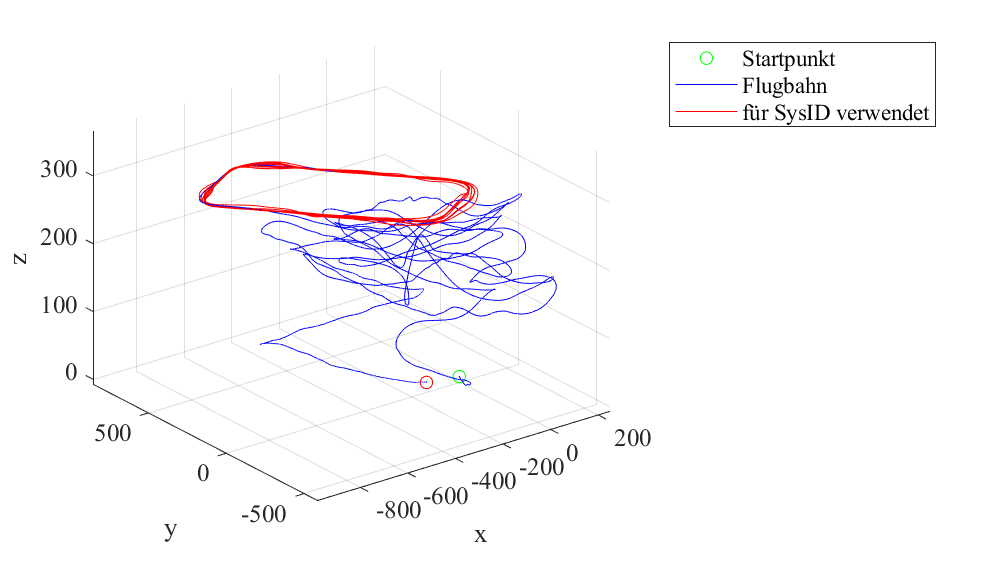
\includegraphics[width=0.9\linewidth]{flug.png}
	\caption{Visualisierung der Flugbahn}
	\label{fig:flug}
\end{figure}

\section{Trimmpunkt} % Fabrizio
In \cref{fig:trimmpunkte} ist beispielhaft der zeitliche Verlauf der Anströmgeschwindigkeit dargestellt. Es zeigen sich 
insgesamt acht stationären Bereiche, die als Trimmpunkt für eine Modellierung dienen könnten. In den nachfolgenden 
Systemidentifikationen soll jeweils der erste Punkt (TP 1) als Grundlage dienen. Dazu werden alle Zustands- und Steuergrößen 
über den Bereich TP 1 gemittelt und diese Mittelwerte als Trimmwerte $ x_0 $ und $ u_0 $ verwendet. Damit lassen sich die 
Abweichungen vom Trimmpunkt berechnen:
\begin{equation}
	\begin{split}
		\Delta x(t) &= x(t)-x_0\\
		\Delta u(t) &= u(t)-u_0
	\end{split}
\end{equation}

Eine Ausnahme bilden hier die Drehraten $ p $, $ q $ und $ r $, bei denen keine Differenz zum Trimmwert gebildet werden muss.


\begin{figure}[h!]
	\centering
	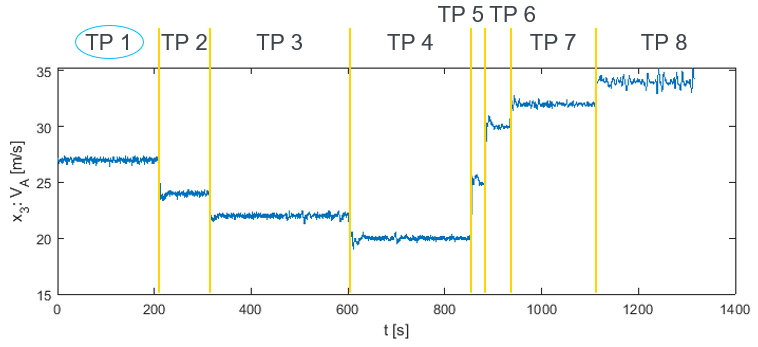
\includegraphics[width=0.9\linewidth]{trimmpunkte.png}
	\caption{zeitlicher Verlauf der Anströmgeschwindigkeit mit den stationären Bereichen}
	\label{fig:trimmpunkte}
\end{figure}




\section{Interpolation} %Florian
Die Rohdaten werden von mehreren Sensoren mit unterschiedlichen Abtastraten geliefert. Da die Identifikationsalgorithmen die 
Werte zu diskreten Zeitpunkten benötigen, ist es notwendig, einen einheitlichen Zeitvektor mit zugehörigen Eingangs- und 
Zustandsvektoren zu generieren. Außerdem wird eine konstante Schrittweite gefordert.\par
Die Abtastrate dieses Zeitvektors ist wichtig, da die Dimension des Optimierungsproblems und damit der 
Rechenaufwand mit feinerer Diskretisierung steigt (im Zeitbereich). In dieser Arbeit wird der Zeitvektor des 

\begin{figure}[h!]
	\centering
	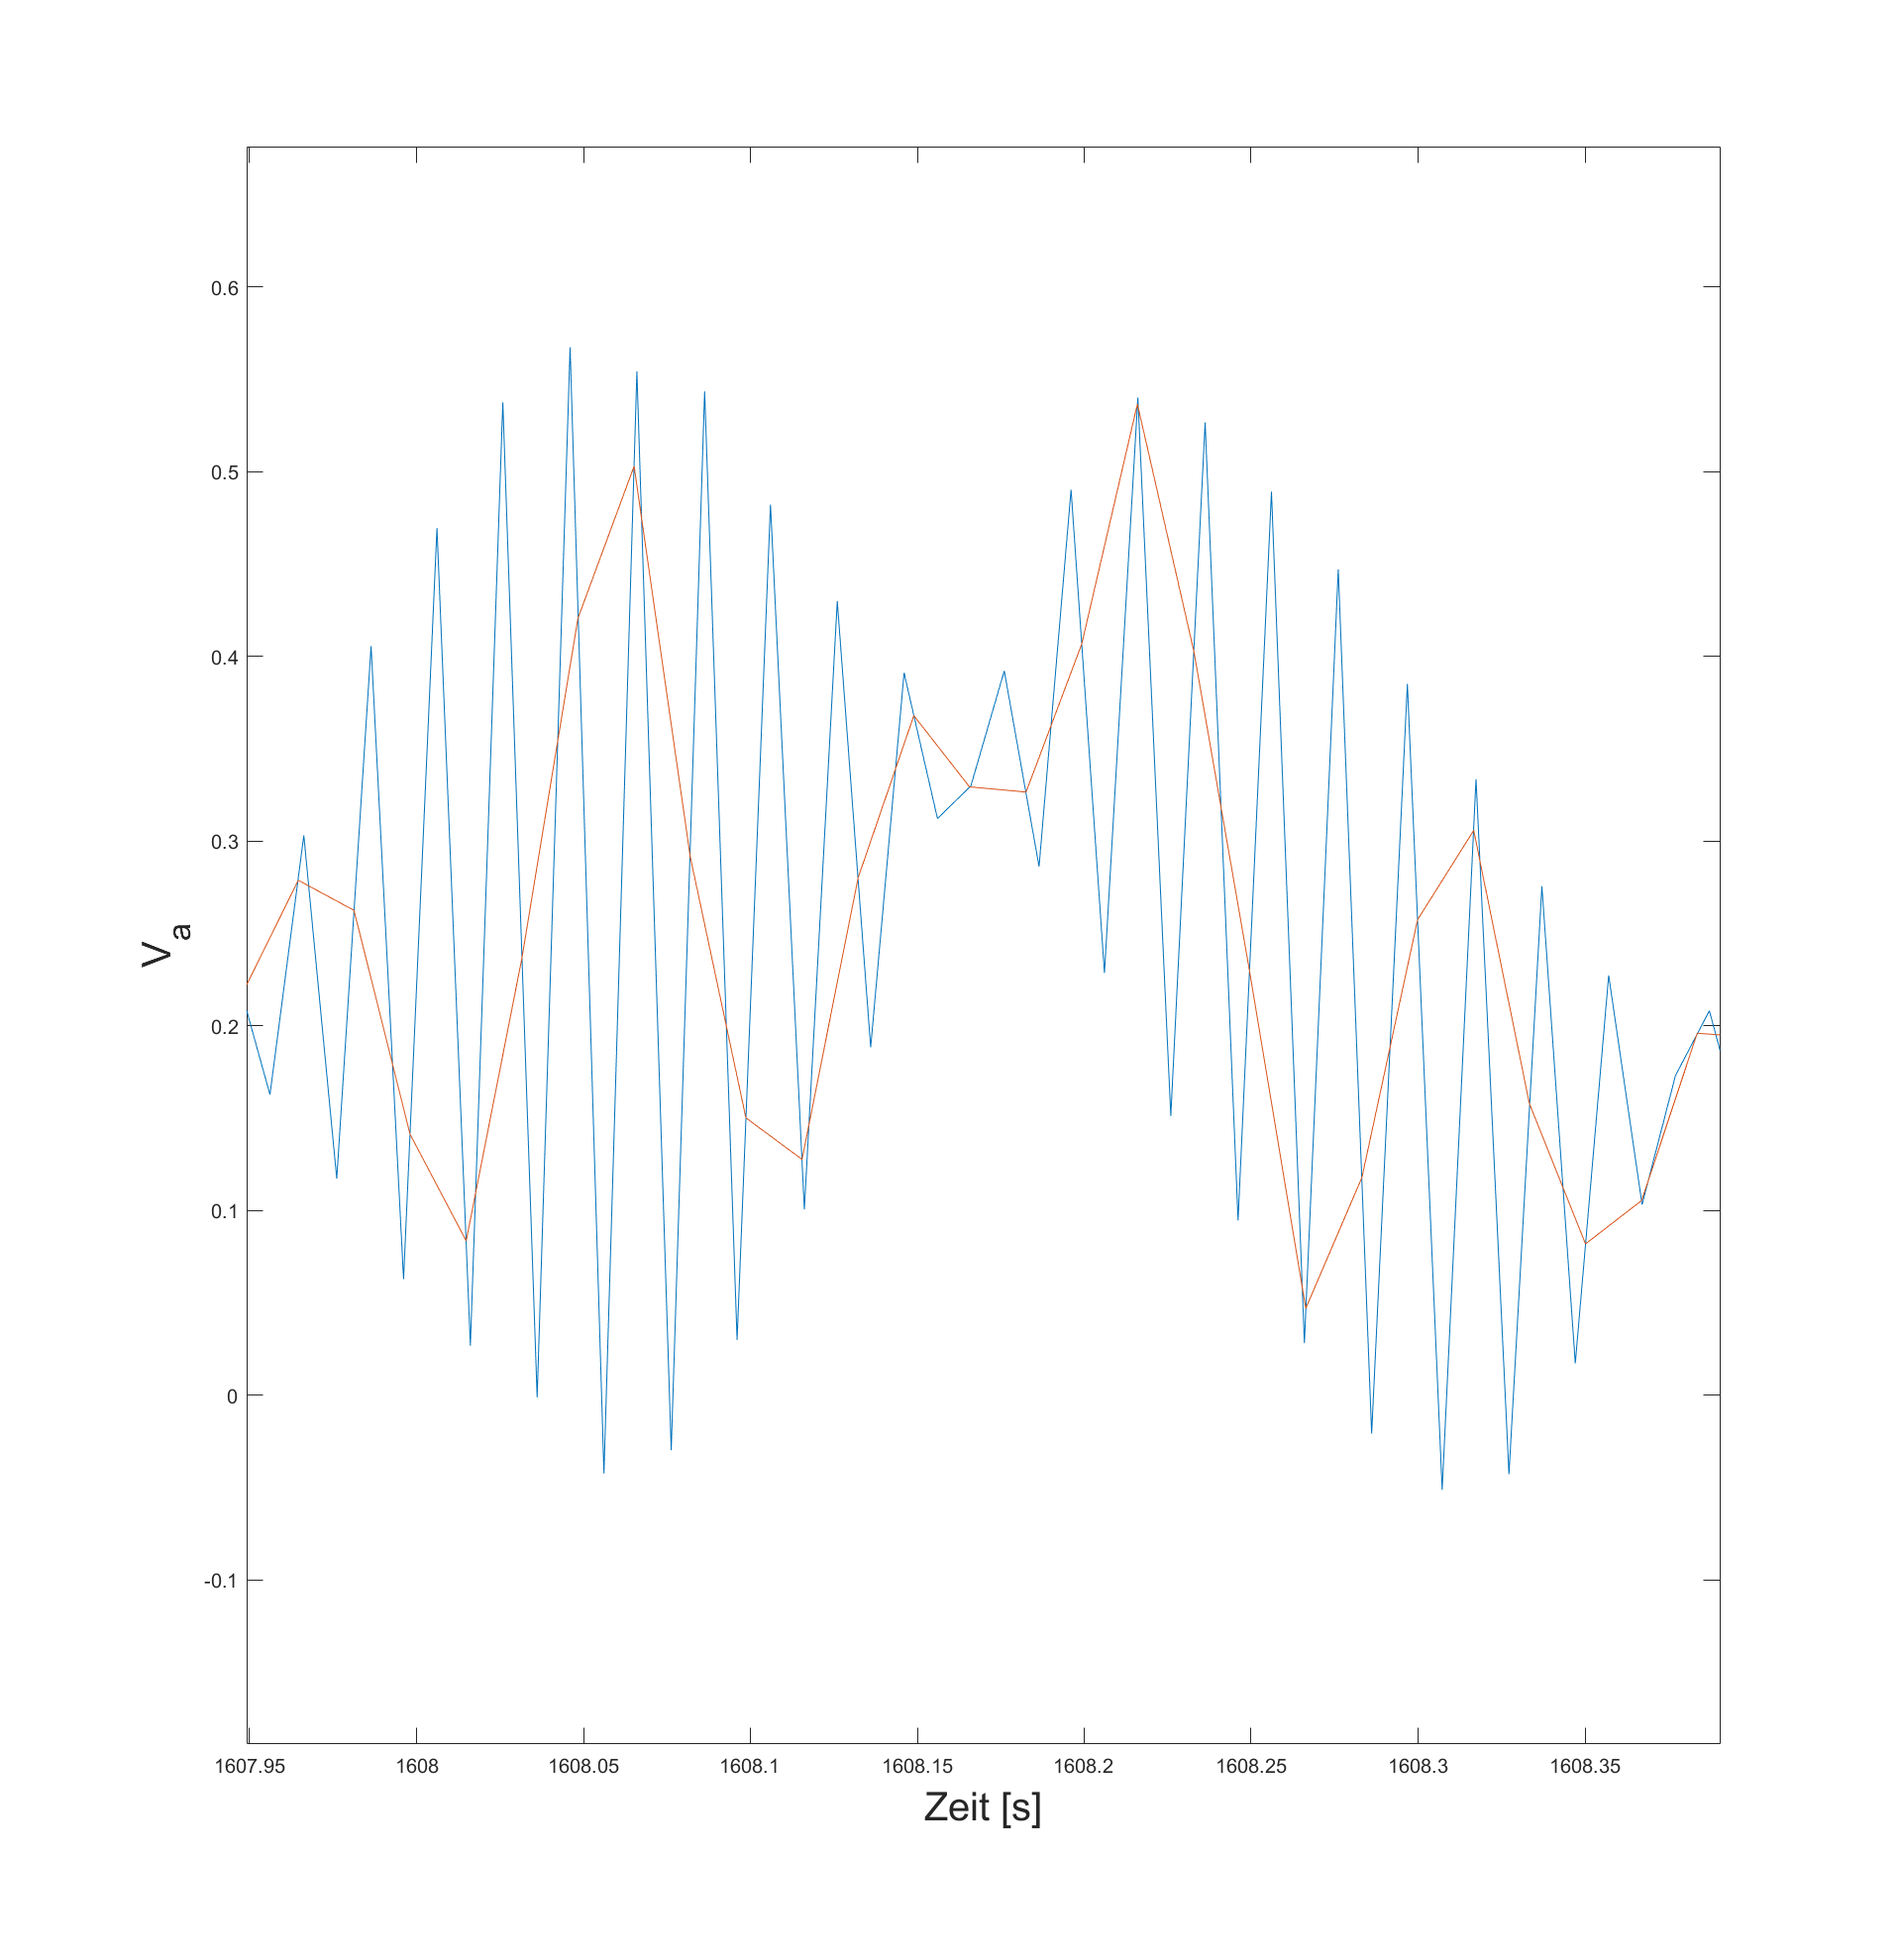
\includegraphics[width=0.7\linewidth]{beispielInterpolation.png}
	\caption{Beispiel Interpolation}
	\label{fig:interpBsp}
\end{figure}

%fkt interp1




\section{Filterung} \label{section:filterung}%Florian
Verrauschte Messdaten stellen für die Systemidentifikation eine Herausforderung dar. Numerische Ableitungen aus verrauschten 
Daten liefern in vielen Fällen keine sinnvolle Aussage. Neben aufwändigeren Ableitungsregeln bietet sich eine vorangehende 
Filterung der Daten an.\par
Das Vorwärts-Rückwärtsfilter bietet den Vorteil, dass keine Phasenverschiebung auftritt. Gerade wenn nur einzelne Signalteile 
gefiltert werden, beispielsweise nur der Eingang, ist diese Eigenschaft unerlässlich. Der Nachteil ist, dass das Filter nicht 
in Echtzeit verwendet werden kann, da immer die vollständige Datenreihe vorliegen muss. Für eine Systemidentifikation ist 
dies jedoch keine praktische Einschränkung.

In \cref{fig:filterBsp} sind die Auswirkungen einer reinen Vorwärts- und einer Vorwärts-Rückwärtsfilterung auf die Phase 
gut zu sehen.

\begin{figure}[h!]
	\centering
	\includegraphics[width=0.7\linewidth]{beispielFilterung.png}
	\caption{Beispiel Filterung}
	\label{fig:filterBsp}
\end{figure}


\subsection{Ablauf}
Für das Filter wird eine Übertragungsfunktion $f(s)$ auf die Messdaten vorwärts 
angewandt, die Messdaten umgekehrt und die selbe Übertragungsfunktion noch 
einmal verwendet. In Matlab ist diese Vorgehensweise in der Funktion \textit{filtfilt()} 
bereits implementiert. 


\subsection{Wahl der Filterübertragungsfunktion}
Es wurde ein quadriertes PT2-Glied gewählt, da so die Eckfrequenz direkt eingestellt werden kann. Die Eckfrequenz wurde zu $ 
\SI{20}{\hertz} $ gewählt, damit das Rauschen unterdrückt wird, aber keine Information verloren geht.

Mit

\begin{equation}
	\omega_{filt} = 2 \cdot \pi \cdot f_{eck} = 2 \cdot \pi \cdot \SI{20}{\hertz}
\end{equation}

%\todo{gewählte Eckfrequenz nennen}

und der Dämpfung

\begin{equation}
	\zeta_{filt} = \frac{1}{\sqrt{2}}
\end{equation}

ergibt sich die Übertragungsfunktion zu:

\begin{equation} \label{eq:filter}
	f(s) = \left(\frac{\omega_{filt}^2}{s^2+2 \cdot \zeta_{filt} \cdot \omega_{filt} +\omega_{filt}^2}\right)^2
\end{equation}

Im Bodediagramm, \cref{fig:bodeplot}, sind Amplituden- und Frequenzgang der Filterfunktion zu sehen.

\begin{figure}[h!]
	\centering
	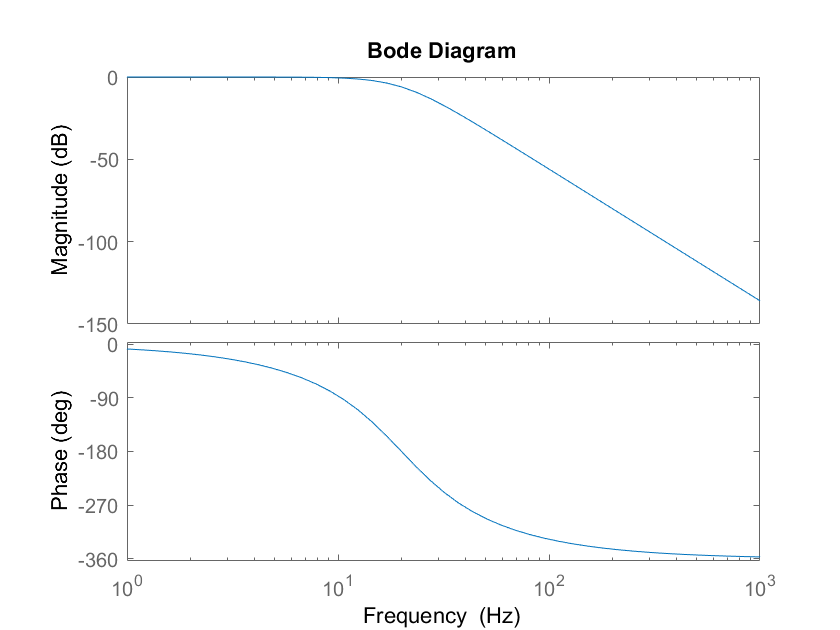
\includegraphics[width=0.7\linewidth]{bodeplot.png}
	\caption{Bodediagramm der Filterfunktion aus \cref{eq:filter}}
	\label{fig:bodeplot}
\end{figure}